\documentclass[12pt,a4paper]{article}

\PassOptionsToPackage{hyphens}{url}

\usepackage[margin=2.5cm]{geometry}
\usepackage{listings}
\usepackage[hidelinks]{hyperref}
\usepackage{cleveref}
\usepackage{multicol}
\usepackage{graphicx}
\usepackage{subcaption}

\begin{document}
\section*{\centerline{COMS32500 - Web Technologies - Website Report}}
\centerline{\small{Lukasz Dygon - ld13281 - May 2016}}
\centerline{\small{Matthew Woodhouse - mw13124 - May 2016}}
\vspace{0.6cm}
\section{Introduction}
Pikchat is an online messenger in which users communicate solely using pictures that they have drawn using the tools provided by the website.
\subsection{Running the Project}
In order to run the project, there are few things which are required to be set up on the server:
\begin{itemize}
\item MongoDB listening on port 27017.
\item Node.js, and 
\item Http-Server (command line http server available from npm) or possibly other HTTP server tool for the front end.
\end{itemize}
To run everything it should be sufficient to execute the following from the /server folder, in the following order:
\begin{enumerate}
\item \texttt{mongod}
\item \texttt{node index} 
\item \texttt{http-server ../client/app}
\end{enumerate}
\section{Client}
The client component of the website uses Bootstrap 3 to provide an underlying framework to allow for fully responsive page layouts. Pages are served using an Angular.js server, which is described in depth in the server section of this report. For the client side, all code was written using the new open source editor by Microsoft, Visual Studio Code (\url{https://github.com/Microsoft/vscode}), which, among other features, provides contextual code completion suggestions aiding in development.For the drawing of input images, the Sketch.js (\url{http://intridea.github.io/sketch.js/}) library was used. This was modified to expand functionality for our needs (clearing the canvas) and to work on mobile devices, although testing on such devices has been limited.

The client should display properly on most modern browsers. Those tested include the latest versions of Chrome, Internet Explorer, Edge, Firefox, and Safari, as well as using the emulated mobile browsers available using the Chrome development tools. We were aiming to support the latest browsers and fail gracefully on slightly older models, which we feel has been achieved, but results on browsers that are significantly older may vary and have not been tested. Standards compliance has been tested, but it is worth noting that due to Angular.js, there are some element attributes that are not considered to be part of the standard. However, without them the backend would not be able to function correctly and as such they have been left in. This does not appear to cause any issues with displaying the web page on any of the browsers used for testing. Aside from this point, the website should be fully standards compliant.
\subsection{HTML}
Main page layout was of course written in HTML. Thanks to the use of Bootstrap, some components were available for us to use and extent, such as the responsive navigation bar. By simply adding divs with the appropriate classes, and then overriding their styling such that they looks as required, components which used to be time consuming to produce can be added with relative ease.

The minimum browser that Bootstrap supports in Internet Explorer 8, and as such our website should function in a reasonable way. Bootstrap also provides an HTML5 shiv, allowing for older browsers to make their best efforts at supporting the newer standard.

Page structure is defined almost exclusively using divs, as these are the most basic building blocks which can be styled to create the desired look using CSS. This was a relatively simple process, as complex pages can be created by nesting and styling divs as required. 

The first page of the website is a splash page of sorts, which provides the option to either log in or register, providing some basic information for new users to get them going. The splash page fills the whole of the browser's view, and then centres the content. All content scales appropriately when viewing on different devices or at different resolutions. In order to log in, an overlay appears over the rest of the page, darkening the inactive content. This was quite difficult to achieve, as it requires a dynamic aspect which is obtained using JavaScript, as described later. In fact, the having content that fills the whole page and works properly at different scales and resolutions can be quite a challenge. A point which caused problems was that when the page scrolled, the background would not cover parts that were not originally visible. This was fixed using a specific nesting of divs, and absolute positioning in the CSS which stretches the background over the whole area.

The rest of the website is composed of a single page with dynamically received content. The top of the page remains the same, and contains a navigation bar and company logo, which can be clicked on to return to the main page. As previous mentioned, the navigation bar collapses into a mobile-style drop down menu when the resolution is below a certain threshold. For messaging and chat, the page then contains a horizontal list of friends. Each of these can be clicked on, and determine the chat that is displayed below. The right hand side of the friends list provides a search bar to allow for filtering. The actual chat section can be switched between the conversation and the user's profile by clicking the buttons to the right of the screen, in line with the user's name.

The profile page displays a list of the images that the user has sent. This makes use of Bootstrap's column system, which divides the page into columns of varied granularity depending on page resolution. This allowed us to create a grid view of images which changes to accommodate different view port sizes.
\subsection{CSS}
Thanks to the use of Bootstrap, a lot of the styling was readily available and could be applied by simply setting the appropriate classes in the HTML. However, to generate our own unique style, these needed to be overwritten using our own custom CSS. This was one of the more challenging areas, as getting the page to look correct in one browser does not guarantee the same for another. As such, a lot of tweaking was required to ensure the pages looked mostly the same across different platforms.

A custom font is also used on the website, 'Roboto', designed and provided by Google. To ensure the font is displayed correctly regardless of whether the client's device has the font installed, it is embedded into the website using the @font-face CSS directive. To ensure that all active browsers are supported, the font is given in a whole host of formats to allow for a consistent viewing experience between devices and browsers. 

The website Font Squirrel (\url{https://www.fontsquirrel.com}) provides a handy 'Webfont Kit', which can be downloaded, already containing the fonts in the required formats and the CSS rules to use them. With minor alterations, they could be used in our website. Font Squirrel also indicates the usage writes for all fonts that it hosts, meaning we were able to make sure the font we chose was used fairly.

An effect which took a surprising amount of time to achieve was having two components next to each other but in the same plane. This was done by floating the components to the left and right, and then additionally placing another div below both with the CSS clear property set to both. This forces the container of the components to actually contain the floated elements, which would otherwise not be considered. Handily, Bootstrap provides a 'clearfix' class which applies exactly the effect, saving us having to define the class ourselves. An example of this in action is the friends bar with the list on the left and search bar on the right.

The positioning of the arrow chat indicator, which points to the appropriate friend, also took some time. To get it in the right position, it needed to be positioned absolutely. This meant that it's container needed to be marked as relative, so that the absolute position was calculated as an offset from its container. The arrow's position is then dynamically set using JavaScript once a friend has been clicked on.

As mentioned in the previous section, getting a full screen overlay is actually quite a complicated process. To stretch over the whole page, there needs to be an outer div with class 'overlay' and an inner div with class 'overlay-wrapper'. The outer div is then positioned absolutely, with all properties (top, left, right, and bottom) being set to zero. This has the effect of stretching over the view port. In order to get anything contained in the overlay to be centred, the inner div is styled such that it has a display property set to table-cell, and vertically align to middle. The outer div is then set to be displayed as table. With this in place, we have an overlay that stretches over the whole screen and any children will be centred both horizontally and vertically. Examples of this are any pop-ups used, such as logging in. The overlay is the translucent black and the child is the login box.

The z-index property also needed to be carefully set. This was relevant because the absolutely positioned elements are by default displayed above others, meaning the drop-down menu was displayed below the friend indicator. Another case where z-index is important is for overlays � these need to be above the rest of the page.

Note that due to the nature of the server, it was in one case required that CSS was directly written into the HTML using $<$style$>$ tags. This is a limitation of the server that we would have hoped to improve upon should more time have been available.
\subsection{JavaScript}
Bootstrap requires jQuery, and as it makes the JavaScript programming process much faster, and provides a lot of additional functionality. Because of this, we also used jQuery for the client side scripting. jQuery uses the same selectors as with CSS, meaning it is possible to apply the same handler to all elements of a single class with only and single function call � a feature made use of by the overlay system.

The first use of jQuery was for displaying and hiding the overlays and message boxes. To display the web page, a click handlers were added to the relevant buttons, which uses the fadeIn() function to show the overlay. By deafult, fadeIn() sets the CSS display property to static, so this was manually overridden to be table, so that the centralisation worked as described in the CSS section. Once the overlay is displayed, it can be dismissed by clicking anywhere outside of the message box. This was done by adding a click handler to the overlay class and calling fadeOut(), and making sure the target of the click event was the overlay and not the message box. This last step was essential, as jQeuery automatically propagates events up from children to their parent. Without it, clicking anywhere in the message box would also dismiss the message. An alternative approach is to use event.stopPropagation(), but this was decided against as it prevented some other features form working as intended due to how the sketching tool works.

jQuery was also used to control the buttons that switch between the chat log and profile for each of the user's friends. This works by toggling the 'disabled� class on and off for both buttons, and fading between the views.

The animation of the pointer was the most involved use of JavaScript for the client. The process for calculating the correct offset is as follows. Firstly, get the position of the friend's image that was clicked, then add half the image's width to get the centre point. The offset of the pointer can then be calculated by taking the previously calculated position, and taking away half of the pointer image's width and also the offset of the pointer's container. This last point is required as the pointer's position is defined relative to its container, and up to this point global coordinates for the whole page were being worked with. This new offset is then passed into the jQuery animate() function, which smoothly transitions the pointer into the correct position.

A small but useful feature of displaying the enhanced image view overlay (zoom in when clicked on) was that the image that needs to be shown can be obtained using purely without having to query the server. As the click handler knows what was clicked on, the function can then get the value of the 'src� attribute of the image in the web page, and then set the image in the overlay to have the same source. While simple, it makes use of the client and removes an unnecessary request to the server.
\subsection{Gimp}
Gimp 2.8 was used to create the image used as the pointer to indicate the currently active chat. It was created by making a transparent image, and using the point-to-point mode of the Free Select tool to select a symmetrical triangle area. The selected area was then filled, ensuring anti-aliasing was enabled in the selection options to ensure there was not a harsh edge. As the background of the image is transparent, the actual colour of the web page it was over would not matter and as such the anti-aliasing would work regardless.

The default profile picture was also created in Gimp. It was made by using the circle select tool to mark out correctly sized regions, then using the flood fill tool to colour them. To get a perfect circle for the head, the Left Shift key is held down while dragging when creating the selection. Each circle made on a separate layer so that they could be moved and aligned correctly.

In addition, the website's favicon was created in Gimp. This was a raster version of the first letter of the full logo that was created in Inkscape, described in the next section. This version was created by filling a circular area with white, then using the correct font to write the letter 'P�, finally moving it into the correct place and flattening the layers before exporting to an icon file.

Due to the nature of our project, most of the images used on the website are generated by the users themselves, and as such there was not a large requirement for bitmap images, leading to few areas where we could highlight our skills with the software without it being unnecessary for the project.
\subsection{Inkscape}
We decided to create our logo in Inkscape, as this allows it to be fully scale invariant due to it being defined as a vector graphic. The SVG is fairly simple, as we wanted to take a modern and flat approach to the website's design, and the logo needed to match this. 

The 'P' of the name was written as a separate text input in Inkscape, and set to be the same red as the navigation's background colour. A near-white circle (matching the website's main page background colour) was placed underneath. This section of the logo was used to make the favicon. The rest of the text in the logo was another text input of the same font. To ensure that the logo would work on all devices regardless of the font being installed, the text was converted to a path using Inkscape's 'Object to Path� tool.
\section{Server}
For development we have used the MEAN stack: MongoDB, Express.js, Angular.js and Node.js.

The node.js server dependencies are listed in the server/package.json.

server/index.js is the main node server script. It connects to the MongoDB server and performs functions including user authentication and authorisation tasks, communication with the server through API and serving content to the client upon valid request. All server side functionality is added to the server upon start.

Required modules are in the /server/node_modules/ folder. Many of them are dependencies of the modules used on the server. /server/package.json specifies dependencies and information about the application.

Express.js is a node framework used to register different API services in the server.

MongoDB was chosen because it has syntax similar to the SQL syntax and allows to change the models quite freely throughout development without breaking the functionality (for example adding and removing columns). It seems to be increasingly used in the technology industry due to its flexibility.

\subsection{Angular.js}
Angular.js is a framework used for creating single page web applications. It achieves it by serving different view and controller at each URL without reloading elements which are kept between each URL (in our case it�s Navbar).

Routing is specified in the /client/app/scripts/app.js. This script also enforces checking of user credentials upon requesting URL access.

The views are defined in the /client/app/views and controllers are defined in the /client/app/scripts/controllers folder.

Restangular is a Rest API service for Angular.js which is used to process http requests to the server and handling responses to create dynamic elements. It is used in our project to receive relevant database elements to be rendered dynamically in the browser. An example  is the messages sent and received by the user from the person they are communicating with. Content of the response is negotiated with the server by making an API call and then using the response to generate the elements in the appropriate view by Angular.js.

\subsection{Authentication and Authorisation}
Passport.js is used for Authentication on the server side. The authentication strategy is set up in the server/passport.js. On the client side the user can register and login.

Angular controllers use authentication service (/client/app/authentication.js) which validates the user and allows requesting registration and login. It handles saving session token in the browser's local storage and whenever authentication is required, it can check whether user is logged in. It also handles logout by deleting session token from the local storage.

Upon registration the server check whether the provided email address is unique. If successful it encrypts the password and saves it in the database. The relevant file is /server/controllers/UserController.js. This also handles login request and issues session token. Token is issued by the server upon successful login and is valid for a day (this value can be easily adjusted).
User cannot proceed to use the tool without being logged in and is automatically redirected to the welcome page once their token cannot be validated.
Some of the authentication infrastructure is similar to the project available at \url{https://github.com/simonholmes/MEAN-stack-authentication/} used to learn how it can be handled. It is however modified quite a bit and it's functionality is extended in our solution.

To register navigate to /#/register or click \"Get Started\" in the homepage and follow instructions on the screen.
To log in click on the \"Log In\" button in the homepage and enter the credentials as indicated.
To log out navigate to /#/pictures or click \"Profile\" in the Navigation Bar, then click \"Logout\" button in the right top corner of the screen.

\subsection{Database} 
As mentioned MongoDB is used as our database. We are using it to store 2 models: 
\begin{itemize}
\item Picture: this includes the png in String format, email address of the sender and email address of the receiver.
\item User: this includes name, email and password encrypted and stored in hash and salt.
\end{itemize}
Client side can communicate with the server side through registered api, allowing it to access and modify contents of the database.

Access to both tables is controlled by server/controllers/PictureController.js and server/controller/UserController.js.

Models are specified inside the /server/models folder.

User models can be accessed by clicking on the profile picture in the Friends bar underneath the Navigation Bar at the /#/home url. This shows conversation with the selected user and allows to view the user gallery by clicking the person glyphicon on the right hand of the screen underneath the Friends bar.

It is also possible to dynamically filter the users displayed by entering part of their email or name in the seatch input box on the upper right side of the screen.

Conversations are produced by accessing the current database of pictures sent between the current user and the user selected in the Friends bar.

To add a picture to the database (and send it to the other user) click on \"New Picture\", draw a picture and press the down arrow button on the top right of the overlay. This should rerender the contents of the chat to include the sent message.

It is possible to delete sent pictures by going to the Profile page (/#/pictures) and clicking on the trash can glyphicon on the bottom right side of the picture. This will prompt the user to confirm the decision and make subsequent request through the API to delete it from the database if decision is confirmed.
\section{Features We Are Proud Of}
Authentication method implemented is relatively complex. It allows safe storage of the passwords and allows people to stay logged in between sessions by the use of the token. This accounts for a better user experience.
Implementing this feature and integrating it with the rest of the system took significant amount of time. The implementation allows for easy expansion into different authentication methods, which is a major consideration in the scalability of the application.
\section{Things that didn't work}
Initially an attmpt was made to implement authentication through use of Kerberos, but it proved difficult. Also it uses a 3rd party authentication. Decision to use passport.js was made and Kerberos authentication was scrapped.

Initially we used Grunt to automate javascript task. It was useful for development, but scrapped due to problems with the portability of the code.
\section{Future Development}
Had more time been available, we would have liked to implement/improve the following features:
\begin{itemize}
\item More advanced user profiles with customisation options such as custom profile pictures.
\item Adding users as friends, instead of everyone being friends with everyone else.
\item Group conversations, involving more than two participants.
\item Custom drawing control, such that the Sketch.js dependency is no longer required and so that we have more control over the element.
\item Provide better information when something goes wrong e.g. logging in failed, registration failed, etc.
\item Using other authentication methods such as Oauth to allow easier access for the users.
\item Enforcing stricter registration rules, with minimum password length and email confirmation to prevent botting.
\end{itemize}
\section{Images}
Should the server prove to be too much hassle to set up, below are some images to show what the website is meant to look like when it is up and running. 
\begin{figure}[h]
\begin{subfigure}[b]{0.5\linewidth}
\centering

\includegraphics[width=0.9\linewidth]{report-img/splash.png}
\caption{Splash Page}
\vspace{4ex}
\end{subfigure}
\begin{subfigure}[b]{0.5\linewidth}
\centering
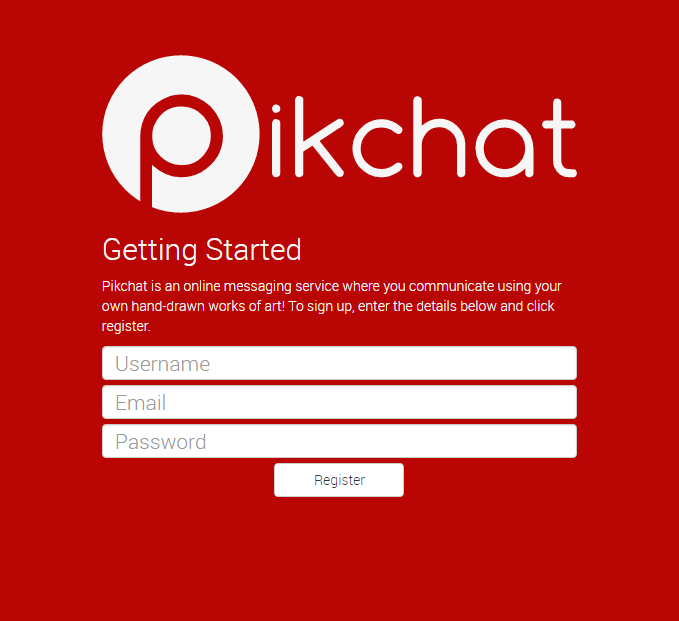
\includegraphics[width=0.9\linewidth]{report-img/register.png}
\caption{Registration Page}
\vspace{4ex}
\end{subfigure}
\begin{subfigure}[b]{0.5\linewidth}
\centering
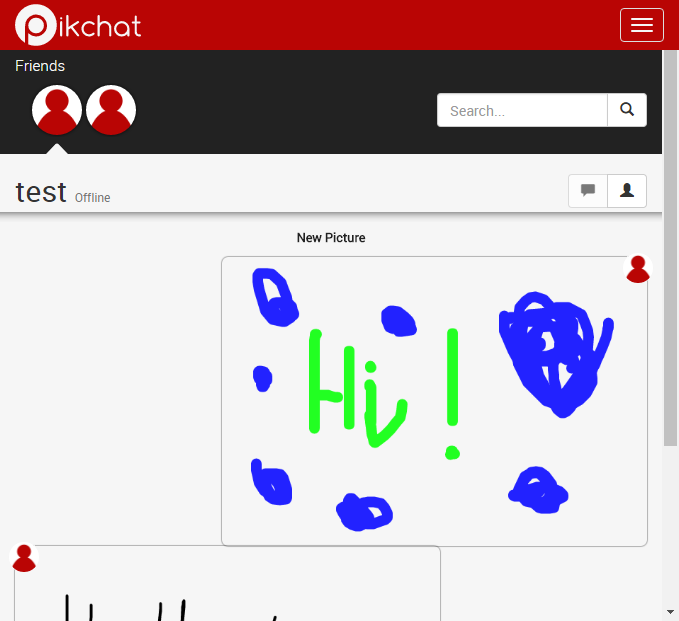
\includegraphics[width=0.9\linewidth]{report-img/main.png}
\caption{Main Page}
\vspace{4ex}
\end{subfigure}
\begin{subfigure}[b]{0.5\linewidth}
\centering
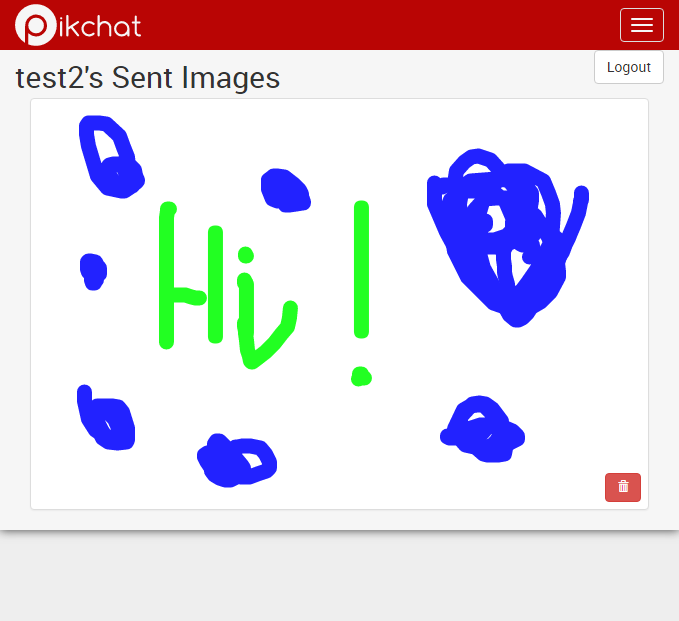
\includegraphics[width=0.9\linewidth]{report-img/profile.png}
\caption{Profile Page}
\vspace{4ex}
\end{subfigure}
\caption{Images showing the website's different pages in action.}
\end{figure}
\end{document}